
%done
Reconstruction from a set of photographs without human assistance is performed in \cite{jan}, they demonstrated the first system able to deliver dense geometry for Internet scale photo collections with millions of images of an entire city within the span of a day on a single PC. They used appearance-based clustering in multiple CPU and GPU cores 
in order agrupate images corresponding to the same site, using gist features for each image along with a RGB
descriptor in order to mantain color information. They also used geo-location information available for some of 
the images. Then at each cluster they performed 3D reconstruction using only the images with mutually consistent epipolar 
geometry. From millions of images from one city they generated thousands of 3D models of buildings. See figure \ref{fig:jan}. 


\begin{figure}[h!]
\begin{center}
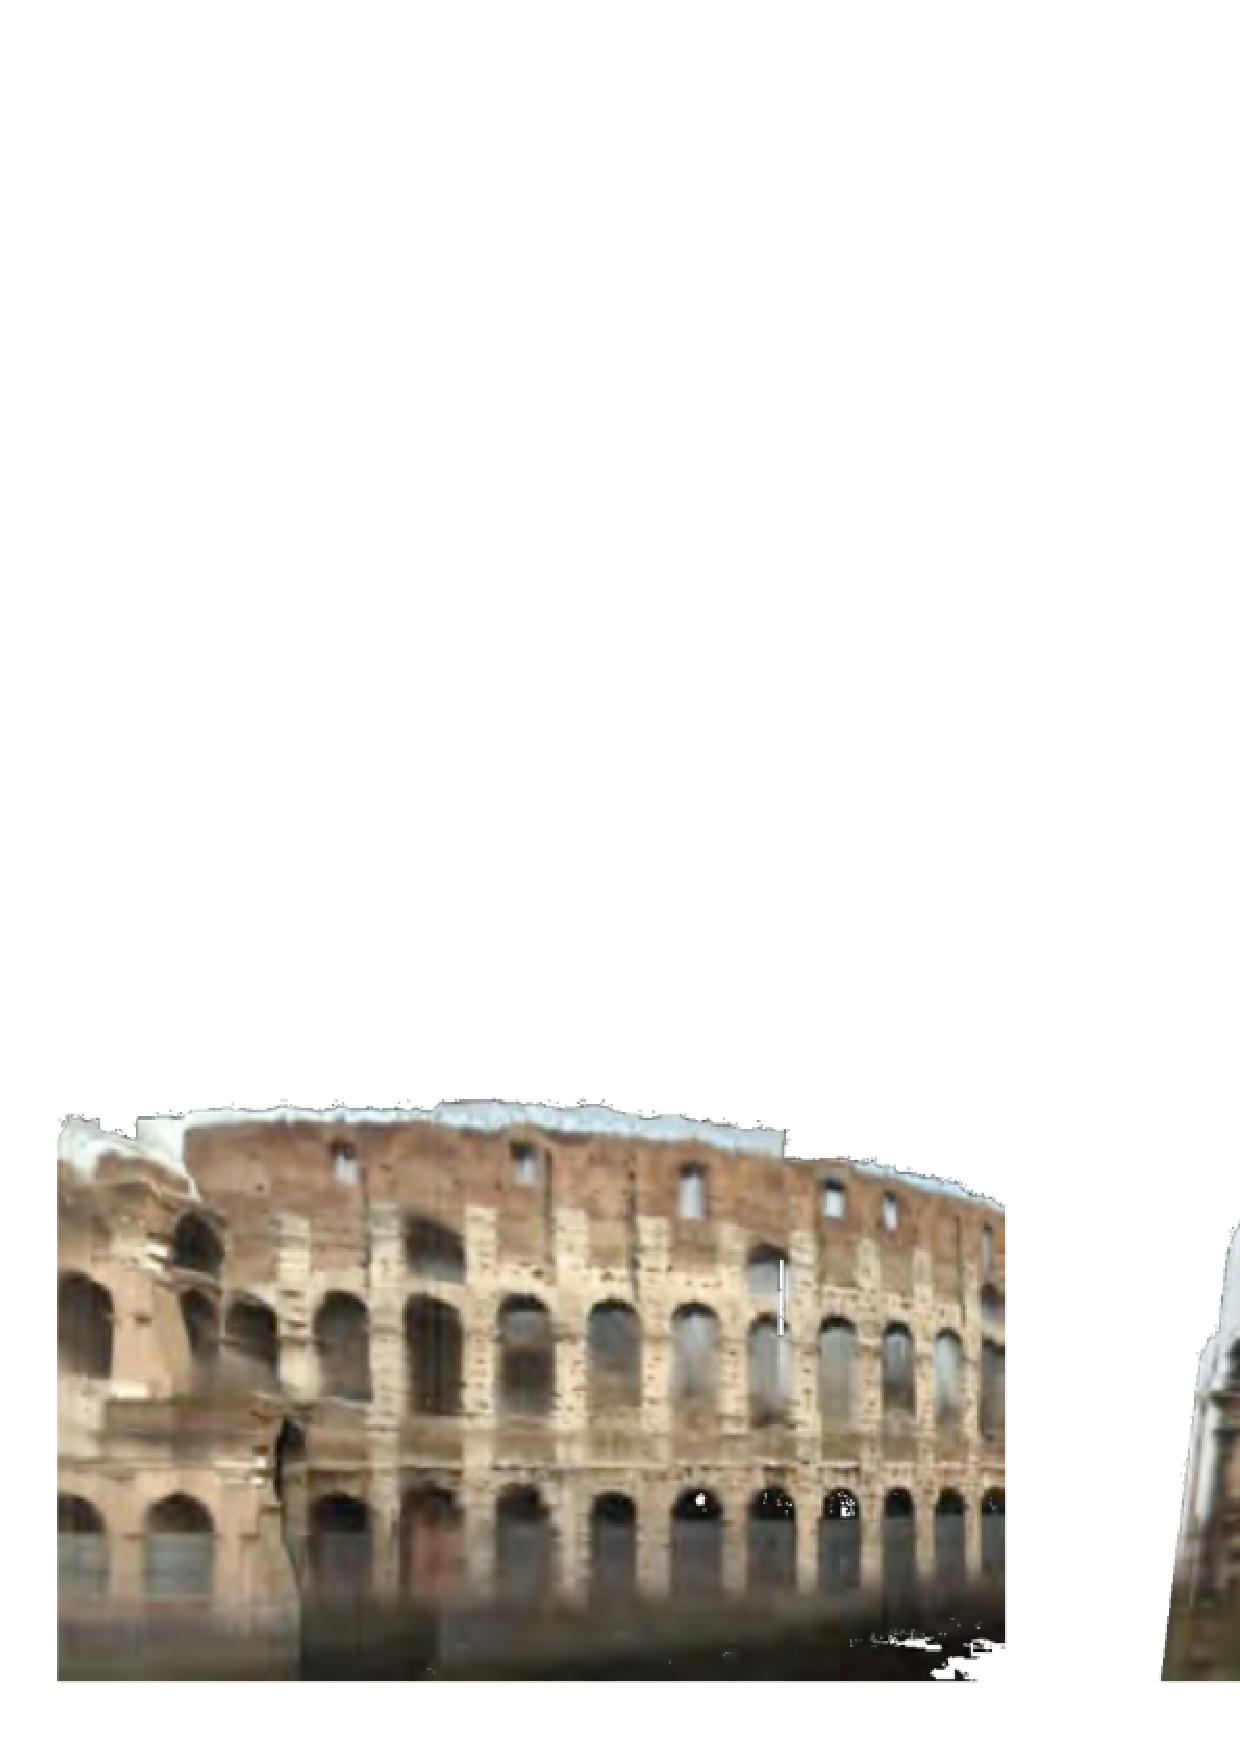
\includegraphics[scale=0.25]{images/jan}
\caption{Reconstructed 3D buildings in less than 24 hr. using 2.8 million and 2.9 million of images respectively}
\label{fig:jan}
\end{center}
\end{figure}


In \cite{guangyu} an hybrid approach is used, combining a ToF camera and an RGB camera in order to perform the reconstruction.
They use a 3D laser scanner in order to obtain a ground truth, obtaining a difference around of 1\% between their reconstructed
 models and the 3D laser models, there are few works were the method is quantitatively evaluated in 3D reconstruction due to the high 
cost of a laser scanner that is used as ground truth. See figure \ref{fig:guangyu}.


\begin{figure}[h!]
\begin{center}
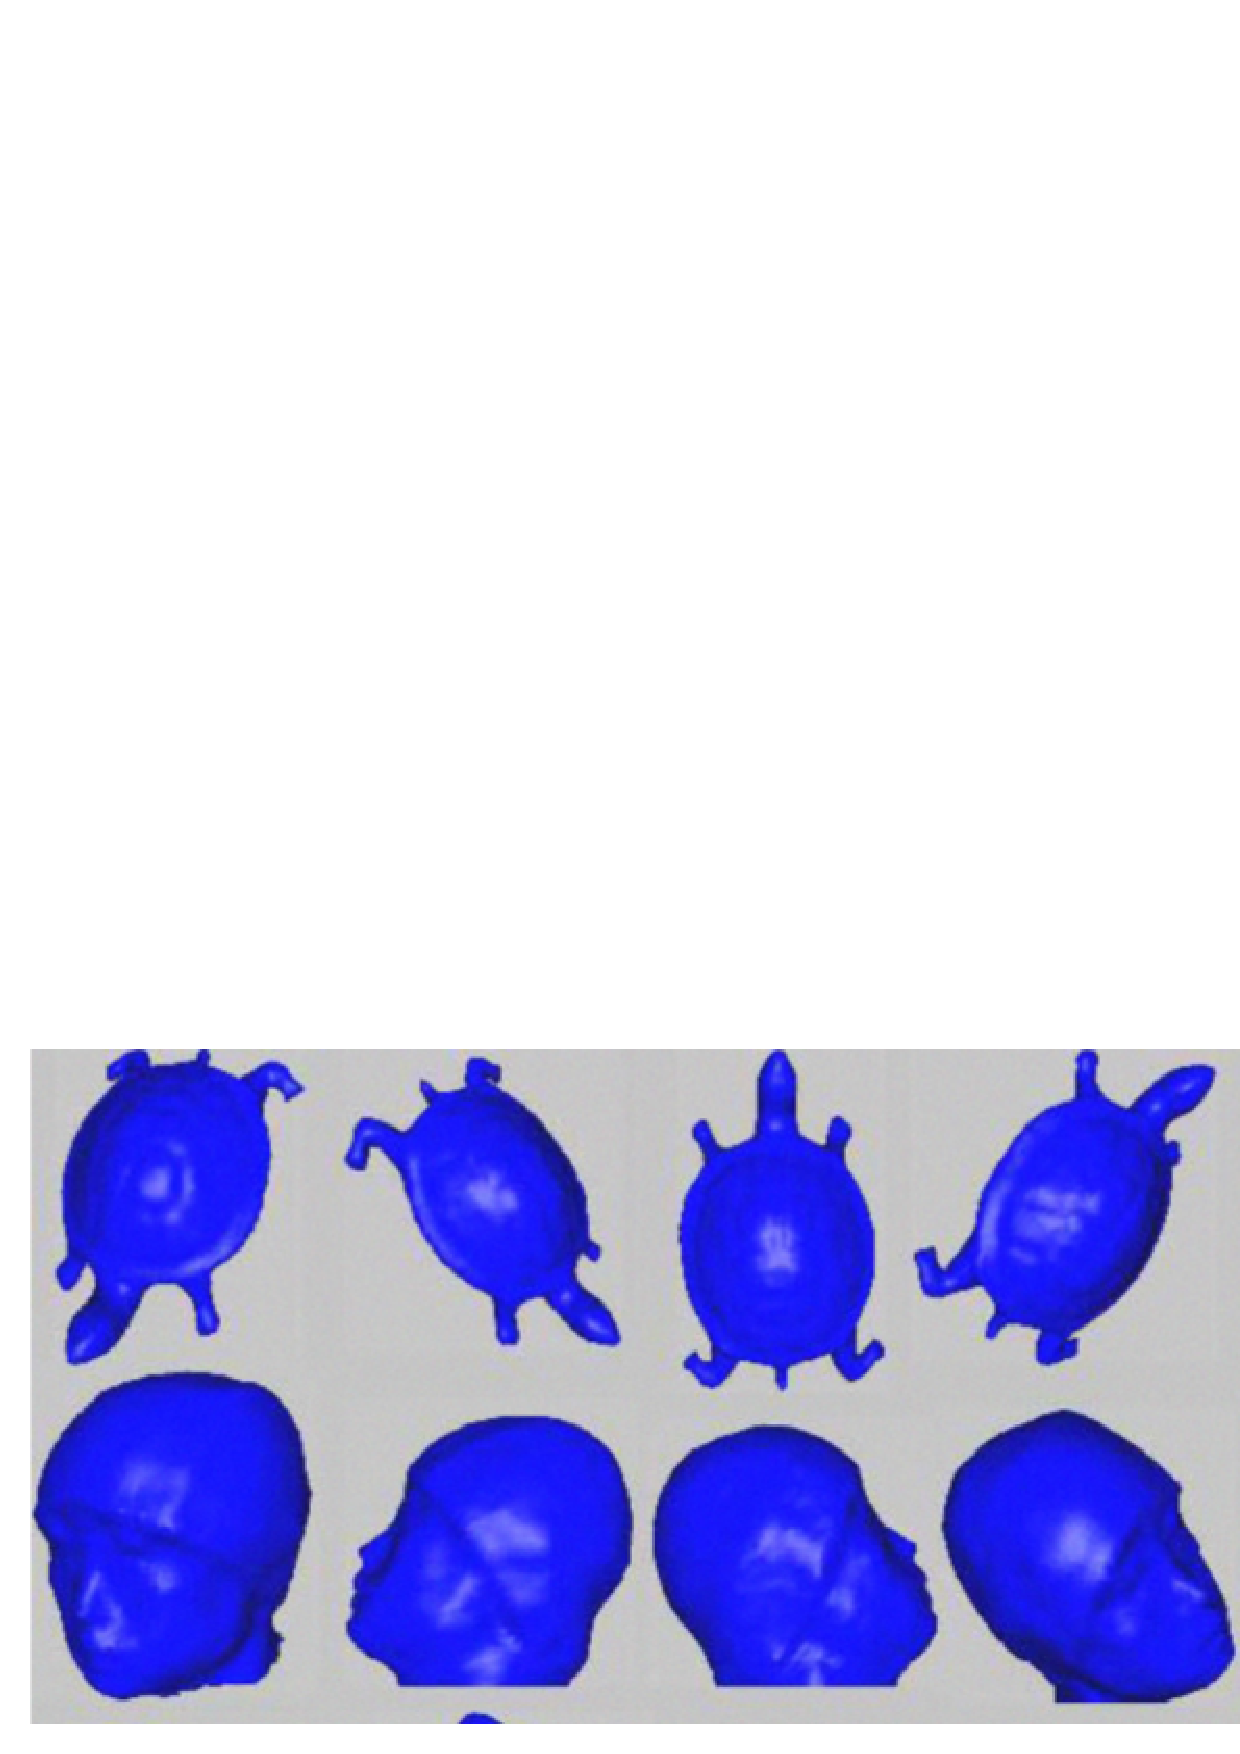
\includegraphics[scale=0.38]{images/guangyu}
\caption{3D Reconstruction of a human head and an object using ToF and RGB camera}
\label{fig:guangyu}
\end{center}
\end{figure}

%done
In \cite{may2009} a ToF camera is used in combination with an industrial robot arm (KUKA KR 16) in order to register an indor scene,
they use an improved version of the ICP algorithm called ICP Frustum, where at each iteration the points that are not overlaping with the previous frame are removed. They use the industrial robot arm to move the camera and get a ground truth camera path to evaluate their camera path estimation.

Its possible to find more elaborated reconstructions using a laser scanner, but its a more expensive method. In 
\cite{binney} there is a interesting work where a reconstruction of tree branches is performed using a laser range 
data. They use a probabilistic approach and use knowledge about the tree structure to guide an iterative reconstruction 
process. In \cite{keqiang} a 3D reconstruction for mobile robots is performed, also with a laser scanner, 
using the ICP algorithm and a volumetric representation.


In \cite{wei} a CCD camera and a 2D laser scanner is used to perform indoor scene reconstruction, they mounted both devices in a rotational stage and use a fusion algorithm to merge the depth map generated by the laser and the depth map generated from the CCD camera observations, the two depth maps contains noise and an intelligent merging reduce this
 noise giving more accurate information to the 3D reconstruction process. Another interesting work of indoor scene reconstruction is \cite{henry} where an RGB-D camera is used to reconstruct an indoor scene. RGB-D cameras are sensing systems that capture RGB images
 along with per pixel depth information. They use the ICP algorithm to calculate the camera location and pass to it information from 
the depth camera and  rich visual
 features along with RANSAC verification captured by the RGB camera. They use surfels \cite{pfister} to represent the scene. See figure \ref{fig:henry}.

\begin{figure}[h!]
\begin{center}
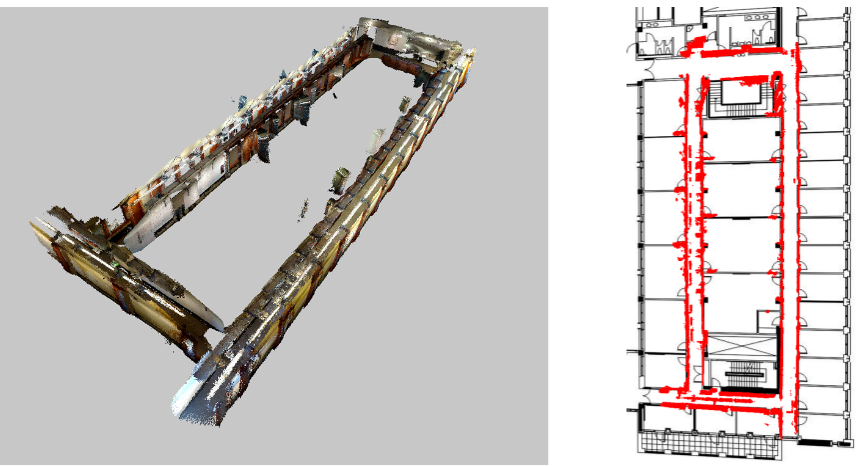
\includegraphics[scale=0.29]{images/henry}
\caption{Reconstructed 3D big indoor space}
\label{fig:henry}
\end{center}
\end{figure}

%done
In \cite{cui} a ToF camera is used to reconstruct 3D objects. A combination of 3D superresolution method with a 
probabilistic scan alignment (iterative Expectation Maximization) approach that takes into account the sensor's 
noise characteristics is used. Their method is not in real time and the resulting models contains undesirable 
artifacts due to  the noise of the captured depth maps, they use a low resolution device (176x144) and they 
improve the resolution using a superresolution method. They captured a ground truth model with a laser 3D scanner, 
obtaining differences below 1 cm in most areas between their model and the ground truth model. Their scanning 
procedure doesn't allow a freely movement around the object, the object must be at the center of view of the camera 
and the distance between the object and camera must be almost constant.
 
see figure \ref{fig:cui}.

\begin{figure}[h!]
\begin{center}
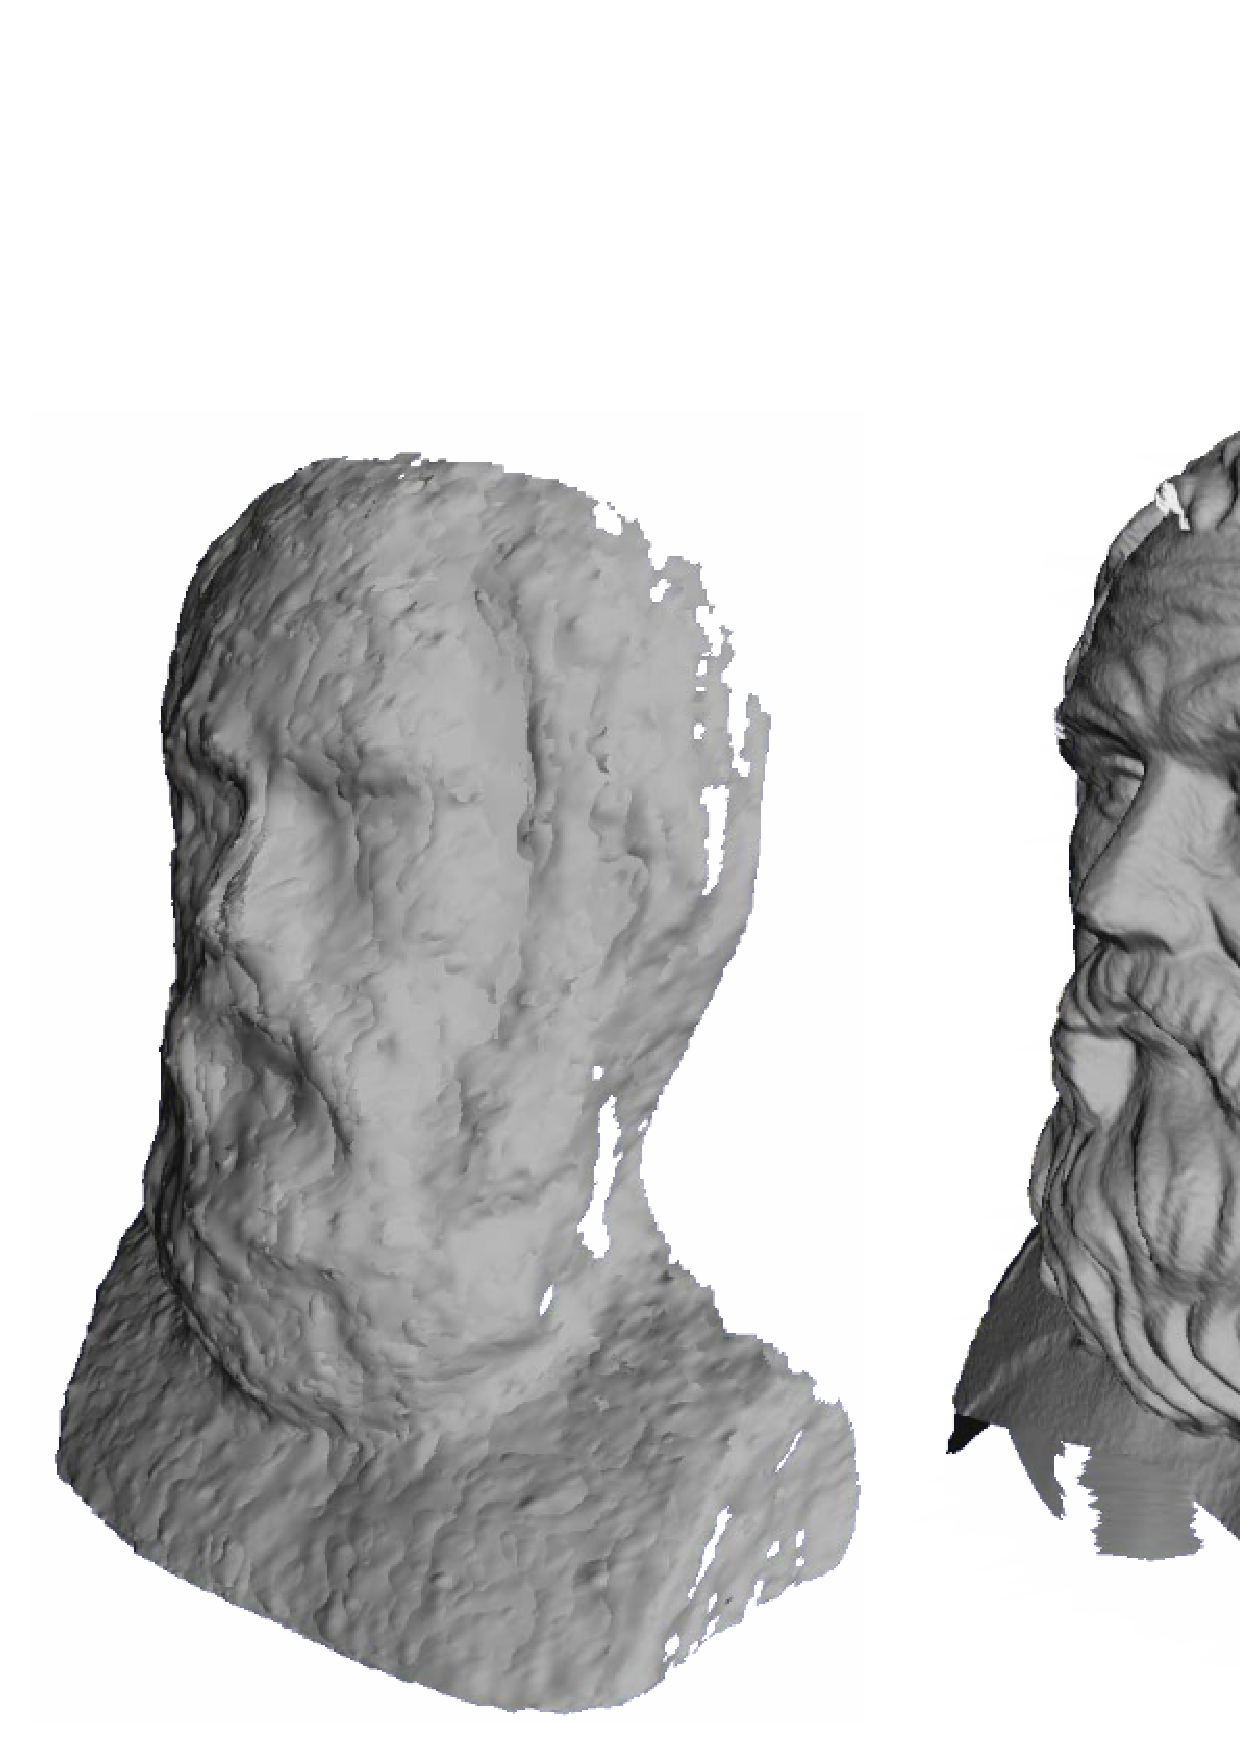
\includegraphics[scale=0.23]{images/cui}
\caption{ToF Reconstruction, Laser Reconstruction and Error Plot}
\label{fig:cui}
\end{center}
\end{figure}

 
%done
A very interesting work is made in \cite{izadi}, they use a low cost RGBD camera (Kinect) in order to perform
the 3D reconstruction using the ICP algorithm  and a volumetric representation with a GPU in order to 
archieve real time reconstruction. The camera can move freely around the scene and the reconstruction grows in detail 
as new depth measurements are added. They apply color textures to the reconstructed scene obtaining very 
realistic models, their system is able to perform rigid body collisions 
simulations during the reconstruction, allowing thousands of virtual particles interact with the scene. Also a 
user can interact with the scene during the reconstruction process. This is one of the most advanced 
reconstruction systems, due to its uniques features.

 see figure \ref{fig:izadi}.

\begin{figure}[h!]
\begin{center}
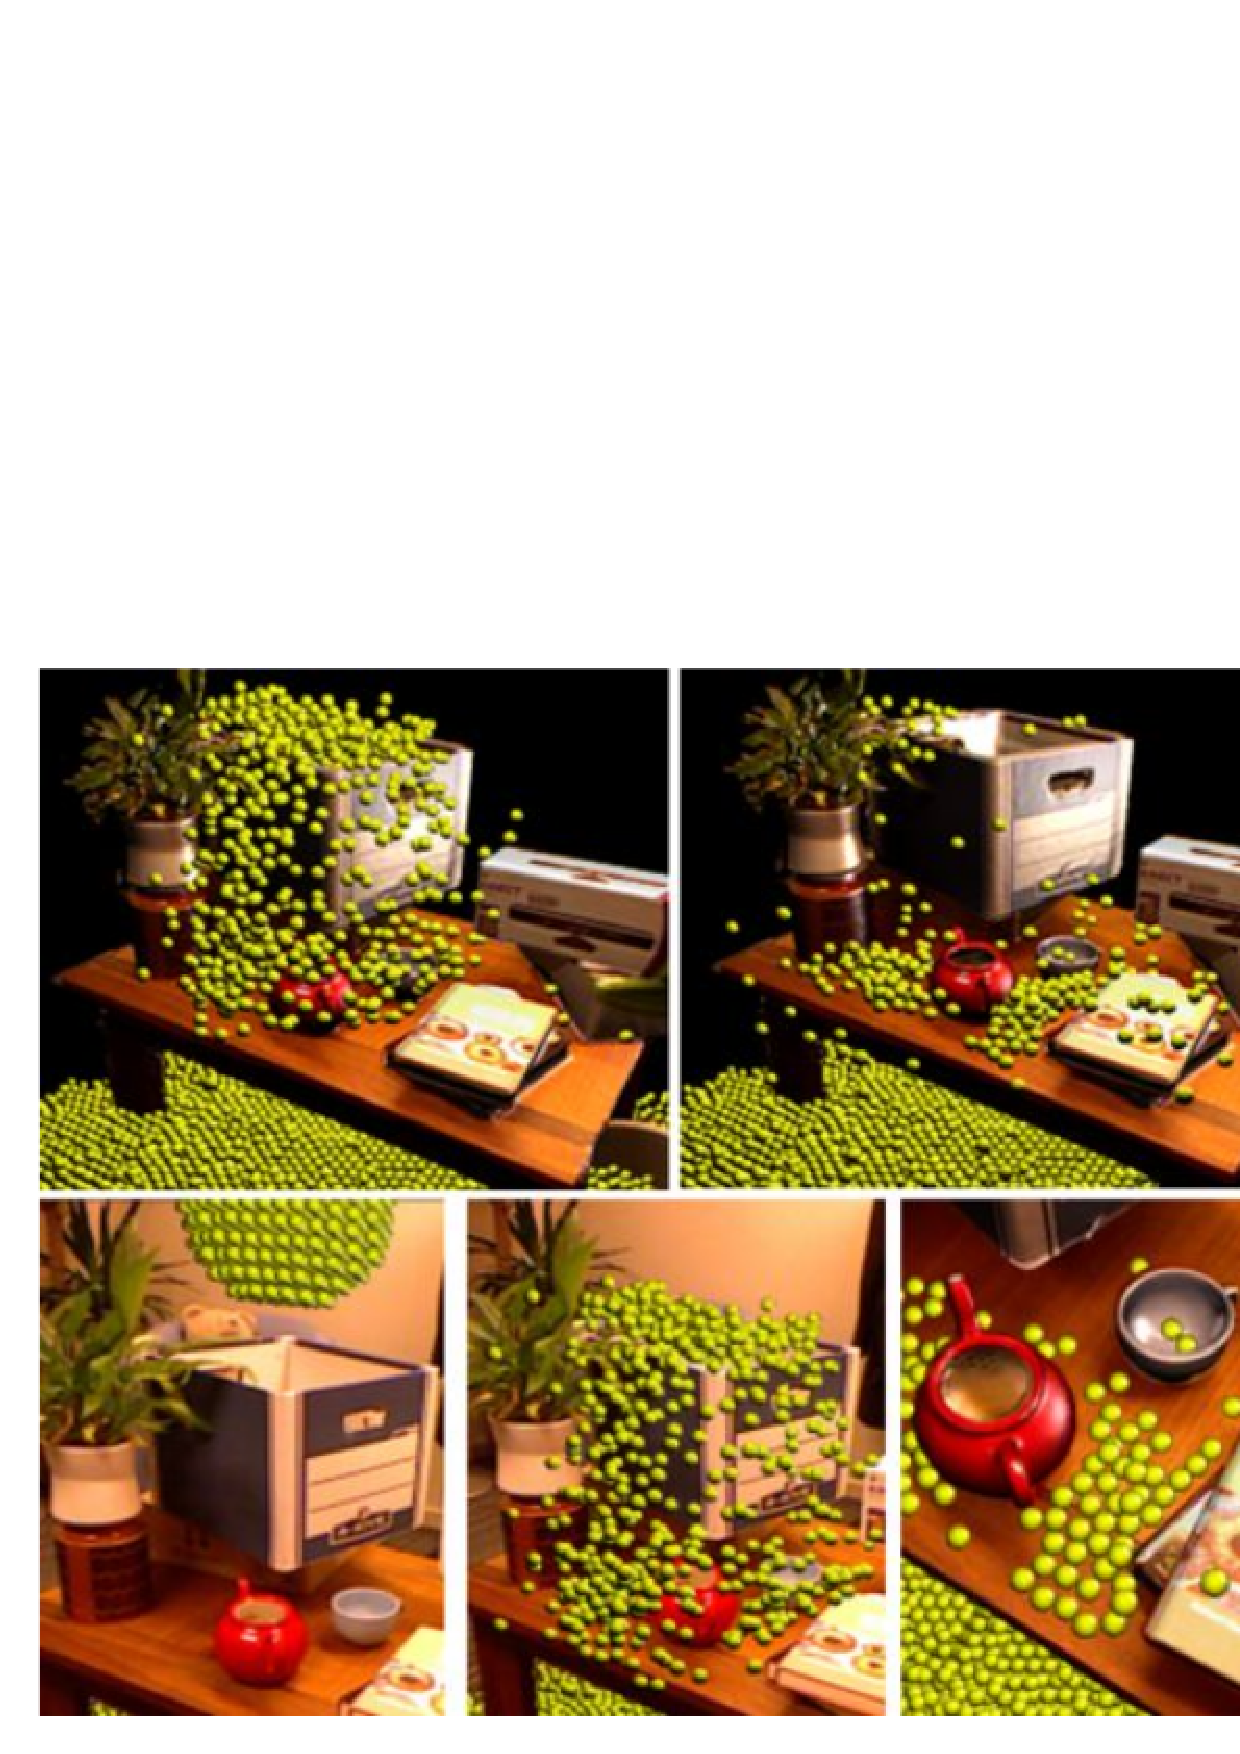
\includegraphics[scale=0.34]{images/izadi}
\caption{Reconstructed 3D scene with thousands of virtual particles}
\label{fig:izadi}
\end{center}
\end{figure}


All the 3D reconstruction methods can have problems with non lambertian 
surfaces and they need to make some assumptions about the surfaces reflectance. For example if we are using an infrared structured light pattern depth camera and the object that we are registering absorbs the infrared light, the reconstruction will fail. Similar problems can occur with laser scanners. Some materials such as glass or water can ruin the reconstruction.
